\documentclass{article}
\usepackage{tikz}
\usepackage{amsmath}
\usepackage{graphicx}
\usepackage[export]{adjustbox}
\usepackage{caption}
\usepackage{subcaption}
\usepackage{listings}
\usepackage{hyperref}
\usepackage{indentfirst}
\usepackage{color} 
\usepackage[utf8]{inputenc}
\usepackage{amsmath}
\usepackage{tikz}
\usepackage{mathtools}
\usepackage{blkarray, bigstrut}
\definecolor{mygreen}{RGB}{28,172,0} % color values Red, Green, Blue
\definecolor{mylilas}{RGB}{170,55,241}
\usepackage{listings}
\usepackage{color}
\usepackage[slovene]{babel}

\graphicspath{ {images/} }

\definecolor{dkgreen}{rgb}{0,0.6,0}
\definecolor{gray}{rgb}{0.5,0.5,0.5}
\definecolor{mauve}{rgb}{0.58,0,0.82}

\newcommand{\tikzmark}[2]{\tikz[overlay,remember picture,baseline] \node [anchor=base] (#1) {$#2$};}

\newcommand{\DrawLine}[3][]{%
  \begin{tikzpicture}[overlay,remember picture]
    \draw[#1] (#2.north) -- (#3.south);
  \end{tikzpicture}
}

\lstset{
  language=Octave,
  aboveskip=3mm,
  belowskip=3mm,
  showstringspaces=false,
  columns=flexible,
  basicstyle={\small\ttfamily},
  numbers=none,
  numberstyle=\tiny\color{gray},
  keywordstyle=\color{blue},
  commentstyle=\color{dkgreen},
  stringstyle=\color{mauve},
  breaklines=true,
  breakatwhitespace=true,
  tabsize=3
}


\graphicspath{ {images/} }
\begin{document}
\pagenumbering{gobble} 
\begin{titlepage}
\author{Domen Gašperlin\\Rok Grmek\\Jakob Gaberc Artenjak\\Anže Gregorc\and Matemetično modeliranje, Fakulteta za računalništvo in informatiko}
\title{\textbf{1. projekt\\Iskanje po zbirki dokumentov}}
\date{April, 2017}

\maketitle

\end{titlepage}

\pagenumbering{arabic}  
\section{Opis problema}
Namen projekta je izdelati iskalnik relevantnih dokumentov po ključnih besedah z metodo\textit{ latentnega semantičnega indeksiranja} (LSI), saj so metode, ki izberejo le dokumente, ki vsebujejo natanko iskane besede, precej nenatačne. Ljudje namreč uporabljamo veliko sopomenk, ki jih preproste metode ne povežejo. Metoda LSI zgradi model, ki združuje več besed v pojme in zato najde tudi dokumente, ki so relevantni, pa ne vsebujejo iskalne besede.

Izdelati je potrebno program, ki bo v dani zbirki za dane ključne besede poiskal najbolj relevantne dokumente.

\section{Naloge}
\subsection{Iz zbirke dokumentov zgradite matriko A povezav med besedami in dokumenti.}
\label{sec:matrikaA}

Matrika A:
\begin{equation*}
  \mathbf{A}=
  \begin{blockarray}{*{5}{c} l}
    \begin{block}{*{5}{>{$\footnotesize}c<{$}} l}
      doc1 & doc2 &  &  docD & \\
    \end{block}
    \begin{block}{[*{5}{c}]>{$\footnotesize}l<{$}}
      a_{11}  & a_{12} & \dots           & a_{1D}       & \bigstrut[t]& beseda1 \\
       a_{21} & a_{22} &                    & \bigstrut[t] &                   &   beseda2 \\
      \vdots   &             & \ddots         &                    &                   &   \vdots  \\
      a_{B1} &              &  \bigstrut[t] & a_{BD}       &                   &  besedaB \\
    \end{block}
  \end{blockarray}
\end{equation*}

 Vsak dokument  ima v matriki svoj stolpec, vsaka beseda pa svojo vrstico. Element a\textsubscript{ij} pa je frekvenca i-te besede v j-tem dokumentu.\\*

Postopek gradnje:
\begin{lstlisting}
  number_of_docs = length(file_names);  # shranimo stevilo vseh dokumentov
  all_words = []; # inicializacija polja, ki bo vsebovala vse besede
  num_of_words_in_docs = zeros(1, number_of_docs); # vektor, ki za vsak dokument hrani stevilo vseh besed
  for i = 1:number_of_docs # sprehodimo se po vseh dokumentih
     # preberemo i-ti dokument
    doc = textread([path_to_docs, filesep, file_names{i}], '%s');
    # vse besede spremenimo na samo alfa numericne znake in v male crke
    for j = 1:length(doc)
      doc{j} = lower(doc{j}(isalnum(doc{j})));
    end
    # dodamo besede i-tega dokumenta v polje vseh besed
    all_words = [all_words; doc]; 
    # dodamo stevilo vseh besed v i-tem dokumentu
    num_of_words_in_docs(i) = length(doc); 
  end

\end{lstlisting}
Ko imamo zgrajeno polje vseh besed, moramo odstraniti podvojene besede in s tem ustvarimo polje, ki bo služilo kot stolpec v matriki A.
\begin{lstlisting}
[unique_words, ~, numbers] = unique(all_words);
\end{lstlisting}

In sedaj imamo vse pripravljeno za gradnjo matrike A:

\begin{lstlisting}
  all_possible_numbers = (1:length(unique_words))';   # vektor od 1 do st vseh unikatnih besed

# matrika A dimenzije (st. vseh unikatnih besed) x (st. vseh dokumentov) 
  A = zeros(length(unique_words), number_of_docs);
  doc_end = 0;

  # sprehodimo se po vseh dokumentih
  for i = 1:number_of_docs
    # hranita stevilo, pri kateri se zacnejo in koncajo besede i-tega dokumenta v polju vseh besed 
    doc_start = doc_end + 1; 
    doc_end = doc_start + num_of_words_in_docs(i) - 1;

    # dodamo frekvence i-tega dokumenta v matriko A
    A(:, i) = histc(numbers(doc_start:doc_end, 1), all_possible_numbers);
  end
\end{lstlisting}

\subsection{Matriko A razcepite z odrezanim SVD razcepom \\
 \( A = U_{k}S_{k}V^{T}_{k} \), ki obdrži le k največjih singularnih vrednosti.}

V Octave okolju lahko odrezan SVD razcep dobimo z ukazom:

\begin{lstlisting}
               [U, S, V] = svds(A, k);
\end{lstlisting}
Odrezan SVD zmanjša t. i. "overfitting" (preveliko prilagoditev modela podatkom, kar povzroči povečan vpliv šuma).

\paragraph{Razmislite kaj predstavljajo stolpci matrike \( U_{k} \) in matrike \( V_{k} \).}
Stolpci matrike \( U_{k} \) predstavljajo "skrite značilnosti" (hidden feature) besed. Ker je matrika ortonormirana, lahko govorimo kot o neki klasifikaciji besed.
Enako velja za matriko  \( V_{k} \), le da njene vrstice predstavljajo "skrite značilnosti" dokumentov.

\paragraph{Kakšen k uporabiti?}
Odločili smo se, da bomo s trisekcijo poiskusili najti najprimernejši k, ki bo ohranil razcep dovolj natančen in obenem zmanjšal vpliv šuma. 
\pagebreak \\
Potek trisekcije: najprej za vsak i od 1 do števila pivotov matrike A izračunamo SVD razcep, ki je odrezan na i največjih singularnih vrednosti. V vektor shranimo logaritemske napake (napaka i-tega razcepa glede na matriko A):

\begin{lstlisting}
svd_errors = zeros(rank(a)-1, 1);
for i=1:length(svd_errors)
	[U, S, V] = svds(a, i);
	svd_errors(i) = log(norm(U*S*V' - a, 'inf'));
end
\end{lstlisting}

Nato s pomočjo trisekcije najdemo dve točki, ki razdelijo podatke (vektor napak) na tri dele. Vsi deli imajo enako število podatkov. Vsako točko posebej pa uporabimo za razdelitev vseh podatkov, po katerih z linearno (\( y = x\cdot b + e \)) metodo najmanjših kvadratov najdemo dve najprimernejši premici. Postopek trisekcije nadaljujemo tako, da prestavimo skrajno desno oz. levo točko (odvisno, kateri dve premici najbolje opisujeta krivuljo napake). Algoritem končamo, ko sta si skrajni levi in desni točki med seboj oddaljeni za manj kot 2. \\ 

\begin{figure}[h]
    \centering
   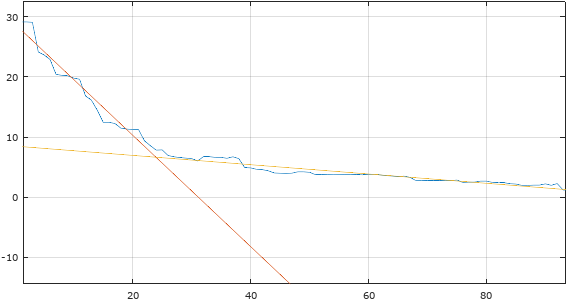
\includegraphics[width=\textwidth]{graf001}
    \caption{x os označuje število k, y os pa logaritemsko napako. Z modro barvo so predstavljeni vsi podatki (napake), rdeča in rumena pa sta premici, ki najbolje opisujeta podatke. }
    \label{slika:trisekcija1}
\end{figure}

Kot se vidi na sliki \ref{slika:trisekcija1}, je dobro vzeti tak k, ki je blizu presečišča premic. Mi smo se odločili, da bomo za k vzeli srednjo vrednost mejnih točk naše trisekcije. Tak k naredi razcep dovolj oddaljen matriki A, torej smo z njim odstranili odvečno prilagoditev modela podatkom, in še vedno dovolj blizu, da lahko pri poizvedbi vrne primerne rezultate. \\

\pagebreak

Implementacija trisekcije:

\begin{lstlisting}
left_limit = 1; # skrajno leva tocka
right_limit = length(svd_errors); # skrajno desna tocka
while(right_limit - left_limit > 2)
	# tocki, ki razdelita podatke na 3 dele
	left = round(left_limit + (right_limit - left_limit) / 3);
	right = round(right_limit - (right_limit - left_limit) / 3);
  
	# z metodo najmanjsih kvadratov izracunani premici, ko so podakti razdeljeni po levi tocki
	[~, ~, r1_left] = ols(svd_errors(1:left), [(1:left)', ones(left, 1)]);
	[~, ~, r2_left] = ols(svd_errors(left:length(svd_errors)), 
      [(left:length(svd_errors))', ones(1+length(svd_errors)-left, 1)]);
	
  	# enako velja za desno tocko
  	[~, ~, r1_right]=ols(svd_errors(1:right),[(1:right)', ones(right)]);
	[~, ~, r2_right]=ols(svd_errors(right:length(svd_errors)), 
      [(right:length(svd_errors))',ones(1+length(svd_errors)-right,1)]);
  
  	# prestavimo skrajno desno oz. levo tocko
	if(mean([r1_left; r2_left].^2) < mean([r1_right; r2_right].^2))
		right_limit = right;
	else
		left_limit = left;
	end
end
k = round((right_limit + left_limit) / 2)
\end{lstlisting}


\subsection{Iskani niz besed (poizvedbo) zapišite z vektorjem q. Iz poizvedbe q generirajte vektor v prostoru dokumentov s formulo 
\( \hat q  = q ^{T}\cdot U_{k}  \cdot S_{ k }^{-1}\) }

Vektor q ima dimenzije enake vektorju, ki vsebuje vse unikatne besede. Zgrajen pa je tako, da je vrstica besede, ki ni v nizu besed (poizvedbi), enaka 0. Vrstice besed, ki pa so vsebovane v poizvedbi pa nosijo vrednost frekvenc določene besede v nizu. Postopek je podoben generiranju frekvenc (stolpcev) za vsak dokument pri nalogi \ref{sec:matrikaA}.

\begin{lstlisting}
q = zeros(length(unique_words), 1);
for i = 2:length(args)
	q += ismember(unique_words, lower(args{i}(isalnum(args{i}))));
end
\end{lstlisting}

Iskanim dokumentom ustrezajo vrstice \( V_{k} \), ki so dovolj blizu vektorju \(  \hat q \). Kot je v navodilih pisalo, smo za razdaljo uporabili kosinus kota med vektorjem \(  \hat q \) in vrsticami \( V_{k} \)  in ne Evklidske razdalje med njima.

\begin{lstlisting}
q2 = q' * U * inv(S); # generiran vektor v prostoru dokumentov

# izracun kosinusne razdalje
cos = (V * q2') ./ (sqrt(sum(q2.^2)) * sqrt(sum(V.^2, 2)));

# vrne vektor relevantnih dokumentov, ki so blizje od min_cos
relevant_docs=sortrows([(1:number_of_docs)', cos](cos > min_cos, :), -2);
doc_names = file_names(relevant_docs(:, 1));
\end{lstlisting}

\subsection{Preiskusite shemo, pri kateri je lokalna mera dana z logaritmom frekvence \( f_{ij} \) i-te besede v j-tem dokumentu: \\*
{\Large\centerline{\( L_{ij} = log(f_{ij} + 1) \)}} \\*
Globalna mera pa je izračunana s pomočjo entropije: \\*
{\Large\centerline{\( G_{i} = 1 - \sum_{j} \frac{p_{ij} \cdot log(p_{ij})}{log(n)}\) } }\\*
kjer je n število dokumentov v zbirki, \\*
{\Large\centerline{\( p_{ij} = \frac{ f_{ij}}{gf_{ij}} \)}}\\*
in \(gf_{ij}\) frekvenca besede v celotni zbirki. }

Metodo je mogoče izboljšati, če frekvence v matriki A nadomestimo z bolj kompleksnimi merami. V splošnem lahko element matrike zapišemo kot produkt
\[ a_{ij} = L_{ij} \cdot G_{i}, \]
 kjer je \(L_{ij} \) lokalna mera za pomembnost besede v posameznem dokumentu, \(G_{i} \) pa globalna mera pomembnosti posamezne besede. \\

Implementacija v Octave:
 \(L_{ij} \) je preprosto samo logaritem matrike A, ki smo jo zgracili pri \ref{sec:matrikaA}:
\begin{lstlisting}
L = log(A + 1);
\end{lstlisting}
\(G_{i} \)  pa generiramo z naslednjii vrsticami:
\begin{lstlisting}
gf=histc(numbers,all_possible_numbers);#frekvenca besede v celotni zbirki
p = f ./ gf; # izracun p-ja
plogp = p .* log(p); # entropija
plogp(isnan(plogp))=0;#ker log(0) vrne NaN, te vrednosti spremenimo na 0
G = 1 - sum(plogp/number_of_docs, 2); # izracun G-ja
\end{lstlisting}
Matrika A pa je potem, kot je bilo že zapisano:
\begin{lstlisting}
A = L .* G;
\end{lstlisting}
Podroben postopek je opisan tudi tukaj: \cite{dumais}

\subsection{Dodajanje dokumentov in besed. Razmislite, kako bi v model dodali nov dokument ali besede, ne da bi bilo treba ponovno izračunati SVD razcep matrike A.}

Ko je matrika A dovolj velika, t. j. ima veliko število unikatnih besed, lahko v model dodamo nove dokumente brez SVD razcepa, saj dokument ne prinaša veliko novih značilnosti in s tem ne vpliva veliko na razcep. Drugače povedano, SVD razcep se ne oddalji od matrike A preveč (napaka se ne spremeni bistveno). \\ \\
Ideja je, da matriki A dodamo nov stolpec (v nadaljevanju vektor d):
\begin{equation*}
  \mathbf{A}=
  \begin{blockarray}{*{6}{c} l}
    \begin{block}{*{6}{>{$\footnotesize}c<{$}} l}
      doc1 & doc2 &  &  docD & docNov \\
    \end{block}
    \begin{block}{[*{6}{c}]>{$\footnotesize}l<{$}}
      a_{11}  & a_{12} & \dots           & a_{1D}       & a_{1D+1}  &  & beseda1 \\
       a_{21} & a_{22} &                    & \bigstrut[t] &  a_{2D+1} &  &  beseda2 \\
      \vdots   &             & \ddots         &                    &  \vdots       &  &   \vdots  \\
      a_{B1} &              &  \bigstrut[t] & a_{BD}       &  a_{BD+1} &  &  besedaB \\
    \end{block}
  \end{blockarray}
\end{equation*}

In ker je \( U \cdot S \cdot V^{T} = A \), in ker želimo v razcep dodati samo vektor d iz matrike A, se ta doda v nov zadnji stolpec (vektor p) matrike \(  V^{T} \):

\[ 
U \cdot S \cdot p = d \]
\[ S \cdot p = U^{T} \cdot d   \]
\[ p = S^{-1} \cdot  U^{T} \cdot d  \]

\section{Uporabniški vmesnik}
Naredili smo tudi uporabniški vmesnik, ki ponuja uporabniku tako generiranje matrike iz dokumentov, kot tudi iskanje po njem. Glavne funkcionalnosti so predstavljene s slikami:  \ref{slika:UI1}, \ref{slika:UI2}, \ref{slika:UI3}, \ref{slika:UI4}

\begin{figure}[h]
 \centering
    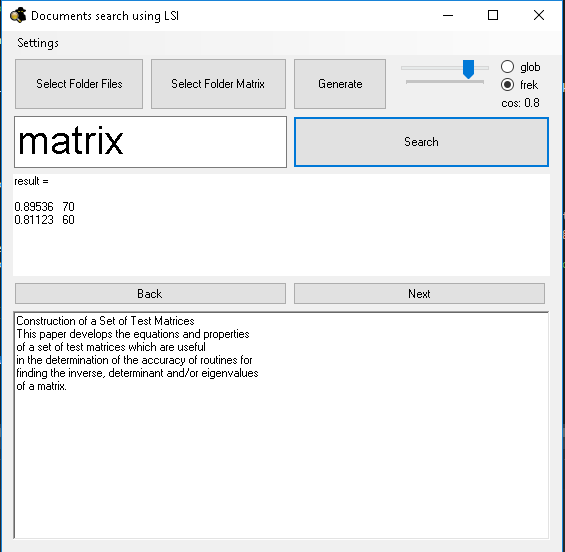
\includegraphics[width=\linewidth]{UI001}
    \caption{Prikazuje iskanje po besedi matrix v datotekah. Rezultat je vrnil dva dokumenta in najbližjega tudi izpisal. }
    \label{slika:UI1}
\end{figure}

\begin{figure}
\begin{minipage}{.5\textwidth}
    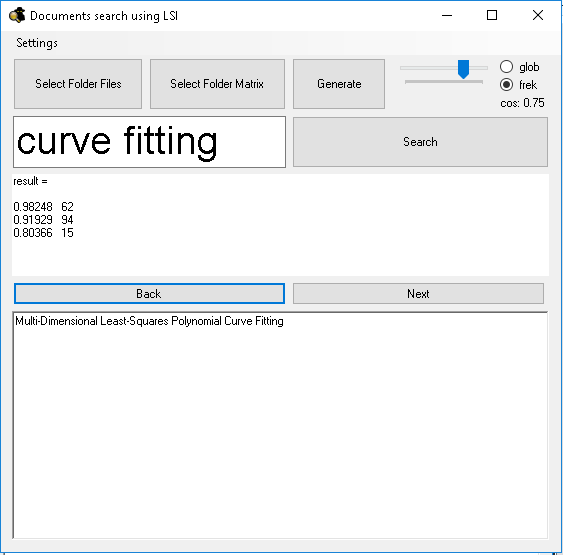
\includegraphics[width=\linewidth,left]{UI002}
    \captionof{figure}{Najbližji dokument }
    \label{slika:UI2}
\end{minipage}%
\begin{minipage}{.5\textwidth}
    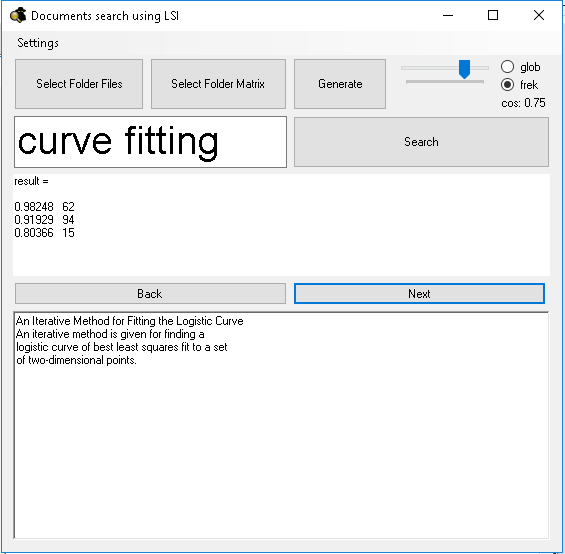
\includegraphics[width=\linewidth,right]{UI003}
    \caption{Drugi najbližji dokument }
    \label{slika:UI3}
\end{minipage} \\
 Poizvedba po nizu 'curve fitting'. S klikom next in back se lahko premikamo po bolj oz. manj dobrih zadetkih. Minimalno kosinusno razdaljo si lahko tudi sami nastavimo (na trenutni sliki je cos: 0.75). 
\end{figure}

\begin{figure}[h]
 \centering
    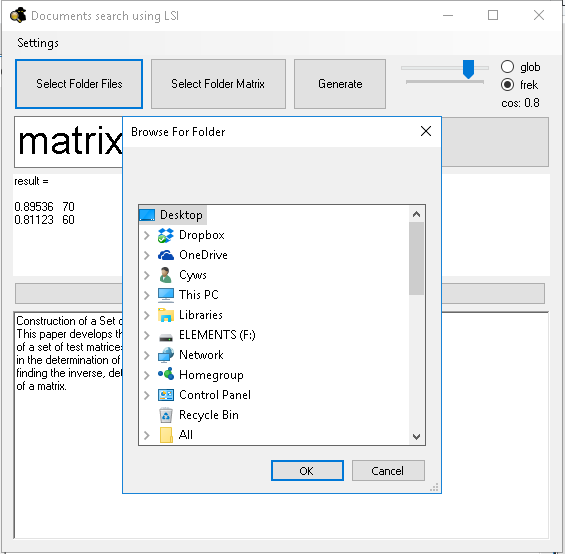
\includegraphics[width=.8\linewidth]{browseDialog}
    \caption{Uporabniški vmesnik omogoča tudi nastavljanje poti do dokumentov.}
    \label{slika:UI4}
\end{figure}


\begin{thebibliography}{9}
\bibitem{dumais} 
Susan T. Dumais. 
\textit{ Improving the retrieval of information from external sources Behavior Research Methods, Instruments,  Computers, 23(2):229–236, 1991.}
\end{thebibliography}

\end{document}